% utf-8 ru, unix eolns
\documentclass[12pt,a4paper,oneside]{extarticle}
    \righthyphenmin=2 %минимально переносится 2 символа %%%
    \sloppy

% Рукопись оформлена в соответствии с правилами оформления 
% электронной версии авторского оригинала, 
% принятыми в Издательстве МГТУ им. Н.Э. Баумана.

\usepackage{geometry} % А4, примерно 28-31 строк(а) на странице 
    \geometry{paper=a4paper}
    \geometry{includehead=false} % Нет верх. колонтитула
    \geometry{includefoot=true}  % Есть номер страницы
    \geometry{bindingoffset=0mm} % Переплет    : 0  мм
    \geometry{top=20mm}          % Поле верхнее: 20 мм
    \geometry{bottom=25mm}       % Поле нижнее : 25 мм 
    \geometry{left=25mm}         % Поле левое  : 25 мм
    \geometry{right=25mm}        % Поле правое : 25 мм
    \geometry{headsep=10mm}  % От края до верх. колонтитула: 10 мм
    \geometry{footskip=20mm} % От края до нижн. колонтитула: 20 мм 

\usepackage{cmap}
\usepackage[T2A]{fontenc} 
\usepackage[utf8x]{inputenc}
\usepackage[english,russian]{babel}
\usepackage{misccorr}

\usepackage{amsmath}
\usepackage{amsfonts}
\usepackage{amssymb}

%\usepackage{cm-super} %человеческий рендер русских шрифтов

\setlength{\parindent}{1.25cm}  % Абзацный отступ: 1,25 см
\usepackage{indentfirst}        % 1-й абзац имеет отступ

\usepackage{setspace}   

\onehalfspacing % Полуторный интервал между строками

\makeatletter
\renewcommand{\@oddfoot }{\hfil\thepage\hfil} % Номер стр.
\renewcommand{\@evenfoot}{\hfil\thepage\hfil} % Номер стр.
\renewcommand{\@oddhead }{} % Нет верх. колонтитула
\renewcommand{\@evenhead}{} % Нет верх. колонтитула
\makeatother

\usepackage{fancyvrb}


\usepackage[pdftex]{graphicx}  % поддержка картинок для пдф
\graphicspath{ {./pictures/} }
\usepackage{rotating}
%\DeclareGraphicsExtensions{.jpg,.png}




\renewcommand{\labelenumi}{\theenumi.} %меняет вид нумерованного списка

\usepackage{perpage} %нумерация сносок 
\MakePerPage{footnote}

\usepackage[all]{xy} %поддержка графов

\usepackage{listings} %листинги
% \renewcommand{\lstlistingname}{Листинг}
% \lstset{
%   basicstyle=\tiny,
%   breaklines=true
%   }


\usepackage{url}


\usepackage{tikz} %для рисования графиков
\usepackage{pgfplots}

\usepackage{gensymb}

\usepackage{ccaption}%изменяет подпись к рисунку
\makeatletter 
\renewcommand{\fnum@figure}[1]{Рисунок~\thefigure~---~\sffamily}
\makeatother

\begin{document}
\pgfplotsset{compat=1.8}

\thispagestyle{empty}
\newpage
{
\centering


\textbf{
МОСКОВСКИЙ ГОСУДАРСТВЕННЫЙ ТЕХНИЧЕСКИЙ УНИВЕРСИТЕТ ИМЕНИ Н. Э. БАУМАНА \\
Факультет информатики и систем управления \\
Кафедра теоретической информатики и компьютерных технологий}
\bigskip
\bigskip
\bigskip
\bigskip
\bigskip
\bigskip
\bigskip

\vfill


Лабораторная работа №6 \\
по курсу <<Математическое моделирование>>

\bigskip

{\large <<Моделирование прыжков на батуте>>}
\bigskip

\vfill



\hfill\parbox{4cm} {
Выполнил:\\
студент ИУ9-111 \hfill \\
Выборнов А. И.\hfill \medskip\\
Руководитель:\\
Домрачева А. Б.\hfill
}


\vspace{\fill}

Москва \number\year
\clearpage
}



\clearpage  


\section{Постановка задачи}
    Моделировать прыжок на батуте. Коэффициент упругости батута $k$, масса прыгуна $m$. Считать, что для набора высоты прыгун отталкивается $n$ раз, прыгает в вертикальном направлении. Построить зависимость набранной высоты от количества прыжков.

\section{Построение математической модели}
\label{sec:model}
    Введём энергию $E_{jump}$, которую прыгун тратит при каждом отталкивании.

    С целью упрощения и ввиду того, что для батута задан единственный коэффициент упругости $k$, будем полагать что батут представляет собой пружинную систему с минимальным коэффициентом упругости $k$, где за место груза - прыгун. Каждый новый прыжок, будет вызывать всё меньшее смещение батута. Для этого представим батут как пружину с фиксированной длиной $l=1$м, для которой коэффициент упругости изменяется с $k$, когда пружина не сжата до $+\infty$ когда пружина сжата до нуля.

    Функция $f_k(\Delta x)$, задающая изменения коэффициента упругости в зависимости от смещения батута от начального положения показана на рисунке~\ref{pic:graphic}. Выразим функцию, представленную на рисунке, как $f_k(\Delta x) = -\frac{1}{\Delta x - 1} + k - 1$ (Это только один из возможных вариантов).

    \begin{figure}[h!]
        \center
        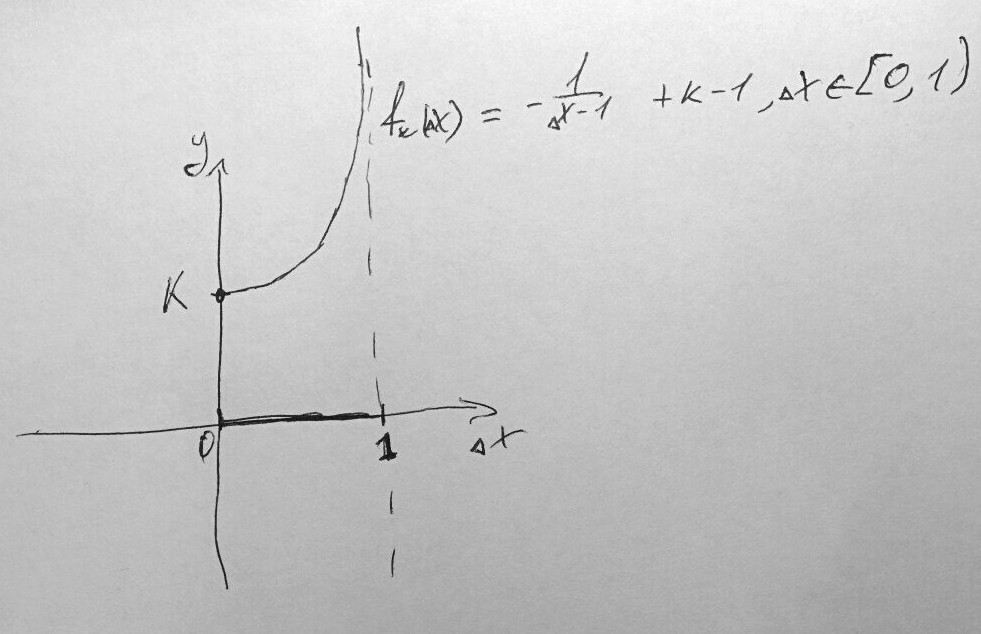
\includegraphics[scale=0.3]{f_k.jpg}
        \caption{График зависимости коэффициент упругости от смежения батута}
        \label{pic:graphic}
    \end{figure}

    Будем считать, что система будет вести себя как пружинный маятник, когда прыгун касается батута. В момент прыжка, он отталкивается от батута и на прыгуна действует только сила тяжести. Когда он приземляется, он тут же снова отталкивается.

    \begin{figure}[h!]
        \center
        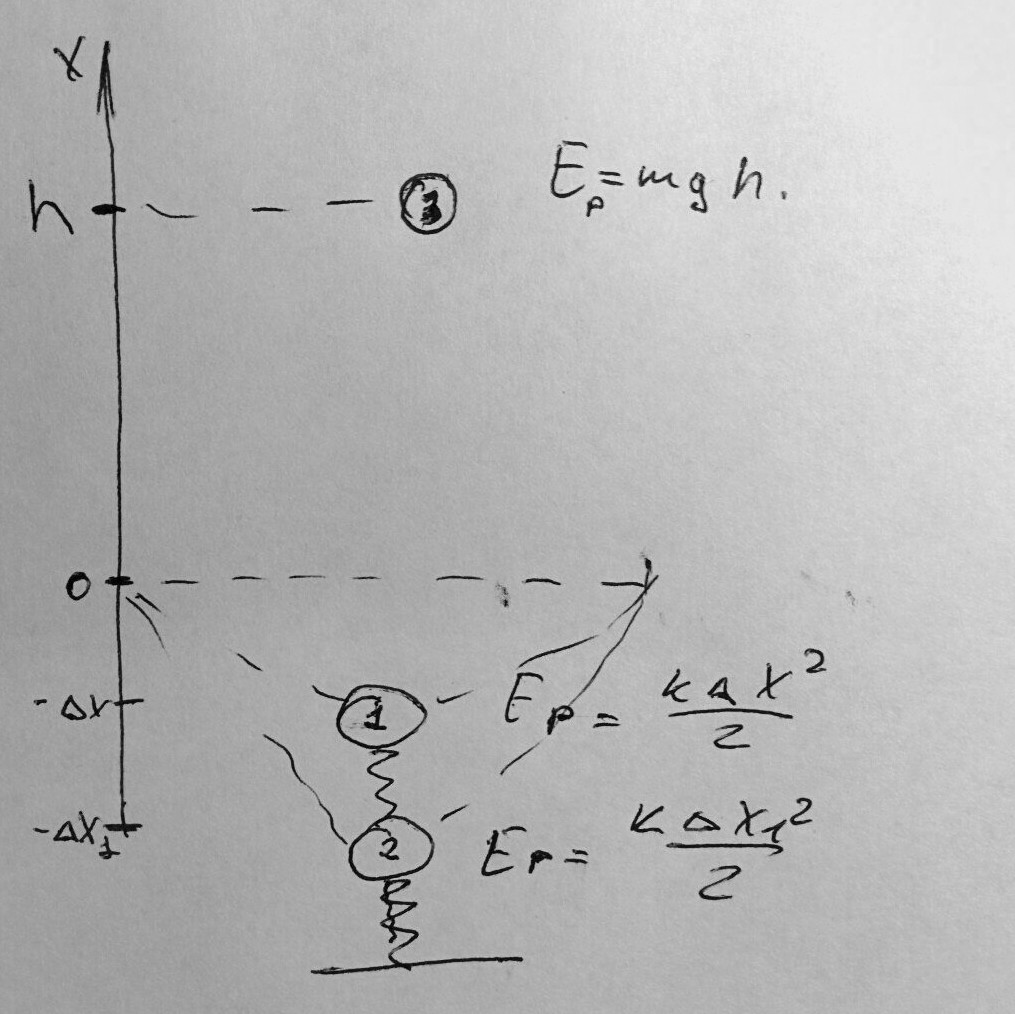
\includegraphics[scale=0.3]{scheme.jpg}
        \caption{Физическая схема задачи}
        \label{pic:scheme}
    \end{figure}

    На вход мы имеем массу прыгуна $m$, функцию, задающую коэффициент упругости батута $f_k(\Delta x)$, энергию отталкивания прыгуна $E_{jump}$, количество толчков $n$. Необходимо найти зависимость высоты прыжка от количества прыжков $h(n)$.

    На рисунке~\ref{pic:scheme} показана схема задачи. Цифрами 1,2,3 - показаны состояния системы. Состояние 1 соответствует моменту приземления, батут сместился на $\Delta x$. Состояние 2 соответствует положению прыгуна сразу после толчка, батут смещён на $\Delta x_1$. Состояние 3 соответствует наивысшей точке, до которой он допрыгнул, прыгун находится на высоте $h$.

    В состоянии 1 система имеет энергию $E_1=\frac{f_k(\Delta x) \Delta x^2}{2}$, затем прыгун затратил энергию $E_{jump}$ на прыжок и переместился в состояние 2. В состоянии 2 система имеет энергию $E_2=\frac{f_k(\Delta x_1) \Delta x_1^2}{2}$.
    То есть совершена работа $E_{jump}$, которая равна изменению энергии системы: $E_2-E_1$. Получили уравнение:
    $$E_{jump} - (\frac{f_k(\Delta x_1) \Delta x_1^2}{2} - \frac{f_k(\Delta x)\Delta x^2}{2}) = 0$$
    Разрешив это уравнение относительно $\Delta x_1$, можно получить значение $\Delta x_1$ по $\Delta x$.
    
    Получили алгоритм, которая позволяющий находить новое смещение батута после прыжка, на основании предыдущего смещения батута.

    Пусть после толчка прыгун находится в состоянии 1, а после того как он подпрыгнул, самый высокой точкой его полёта была точка, соответствующая состоянию 3. В состоянии 3 система имеет энергию $E_3=mgh$. По закону сохранения энергии энергия в состоянии 1 и состоянии 3 равна, то есть:
    $$\frac{f_k(\Delta x) \Delta x^2}{2} = mgh$$
    Выразим высоту:
    $$h(\Delta x) = \frac{f_k(\Delta x)\Delta x^2}{2mg}$$
    Получили зависимость высоты прыжка от смещения батута перед прыжком.

    Теперь мы можем построить итеративный процесс следующий образом: начиная с смещения $\Delta x=0$ симулируем прыжок и получаем новое смещение $\Delta x_1(\Delta x)$. Затем находим высоту прыжка $h(\Delta x_1)$. Присваиваем $\Delta x = \Delta x_1$. Повторяем $n$ раз.
    
\section{Реализация}
    Ниже представлена реализация итеративного алгоритма, описанного в главе~\ref{sec:model}:
    \begin{lstlisting}
    f_k = lambda x: -1/(x-1) + k - 1
    f = lambda dx, dx1: f_k(dx1)*dx1**2 - f_k(dx)*dx**2 - 2*E_jump

    h = lambda dx: k*dx**2*1.0/(2*m*g)
    new_dx = lambda dx: min(
        fsolve(lambda dx1: f(dx, dx1), max(dx, 1e-5))[0],
        1-1e-5
    )

    dx = 0
    for i in range(1, n+1):
        dx = new_dx(dx)

        print dx, h(dx)
    \end{lstlisting}


\section{Результаты работы}
\label{sec:test}
    Программа, описанная выше была запущена с параметрами: $m=80$кг, $k=5000$H/м, $E_{jump}=240$Дж, $n=10$. Полученная зависимость максимальной высоты от количества прыжков изображена на рисунке~\ref{pic:test}. Зависимость смещения батута от количества прыжков представлена на рисунке~\ref{pic:test1}.

        \begin{figure}[h!]        
        \centering
            \begin{tikzpicture}[scale=1]
                \begin{axis}[ ylabel=максимальная высота (м), xlabel=количество прыжков,
                ] 
                    \addplot coordinates {                            
                        (1,0.305782943909)
                        (2,0.611525419757)
                        (3,0.917218776569)
                        (4,1.22284327373)
                        (5,1.52836307191)
                        (6,1.83370921763)
                        (7,2.13873225934)
                        (8,2.4430396743)
                        (9,2.74518363623)
                        (10,3.03357843929)
                        (11,3.18546126433)
                        (12,3.18546126433)
                        (13,3.18546126433)
                        (14,3.18546126433)
                        (15,3.18546126433)
                        (16,3.18546126433)
                        (17,3.18546126433)
                        (18,3.18546126433)
                        (19,3.18546126433)
                        (20,3.18546126433)
                    };
                \end{axis}
            \end{tikzpicture}
        \caption{Зависимость максимальной высоты от количества прыжков}
        \label{pic:test}
        \end{figure}


        \begin{figure}[h!]        
        \centering
            \begin{tikzpicture}[scale=1]
                \begin{axis}[ ylabel=смещение батута (м), xlabel=количество прыжков,
                ] 
                    \addplot coordinates {                            
                        (1,0.309824759747)
                        (2,0.438143880215)
                        (3,0.536594184035)
                        (4,0.619576436358)
                        (5,0.692664230009)
                        (6,0.758708110934)
                        (7,0.819384421901)
                        (8,0.875739124715)
                        (9,0.928314627207)
                        (10,0.975859079818)
                        (11,0.99999)
                        (12,0.99999)
                        (13,0.99999)
                        (14,0.99999)
                        (15,0.99999)
                        (16,0.99999)
                        (17,0.99999)
                        (18,0.99999)
                        (19,0.99999)
                        (20,0.99999)
                    };
                \end{axis}
            \end{tikzpicture}
        \caption{Зависимость смещения батута от количества прыжков}
        \label{pic:test1}
        \end{figure}

\section{Выводы}
    Из результатов работы программы, описанных в главе~\ref{sec:test}, видно что зависимость максимальной высоты прыгуна от количества прыжков линейная, но ограничена максимально возможной ''раскачкой''  батута. Также видно, что с каждым прыжком уменьшается изменение смещения батута.
    
\end{document}